This is another important layer in our design. This part of the system works as a bridge between the User Interface and the Database of the system. If the data is being received from the UI controller that are coming form different subsections of UI, the Business controller will, depending upon what kind of input it gets, either generate an AR, generate a Qr or does an input validation. The Business Logic will send the data to the data base for more validation and verification or to store the data in database. If Business Logic is getting the instruction to fetch data form Database, then it will contact Database to get particular data, which is then passed on to the UI.

\subsection{Layer Hardware}
A description of any involved hardware components for the layer. For example, if each subsystem is a software process running on an embedded computer, discuss the specifics of that device here. Do not list a hardware component that only exists at the subsystem level (include it in the following sections).

\subsection{Layer Operating System}
A description of any operating systems required by the layer.

\subsection{Layer Software Dependencies}
This layer is build using ReactNative. Dependencies we needed for this part are
\begin{rand}"dependencies":\\ {
    "expo": "34.0.1",\\
    "expo-barcode-scanner": "6.0.0",\\
    "expo-permissions": "6.0.0",\\
    "firebase": "6.6.0",\\
    "native-base": "2.13.7",\\
    "react": "16.8.3",\\
    "react-dom": "16.8.6",\\
    "react-native": "https://github.com/expo/react-native/archive/sdk-34.0.0.tar.gz",\\
    "react-native-datepicker": "1.7.2",\\
    "react-native-gesture-handler": "1.4.1",\\
    "react-native-search-bar": "3.4.3",\\
    "react-native-simple-radio-button": "2.7.3",\\
    "react-native-vector-icons": "6.6.0",\\
    "react-native-web": "0.11.4",\\
    "react-navigation": "4.0.0",\\
    "react-navigation-stack": "1.5.1",\\
    "reinput": "3.7.1"]\\
\end{rand}
\subsection{Subsystem 1}
Descibe at a high level the purpose and basic design of this subsystem. Is it a piece of hardware, a class, a web service, or something else? Note that each of the subsystem items below are meant to be specific to that subystem and not a repeat of anything discussed above for the overall layer.

\begin{figure}[h!]
	\centering
 	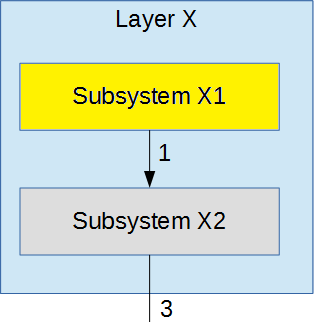
\includegraphics[width=0.60\textwidth]{images/subsystem}
 \caption{Example subsystem description diagram}
\end{figure}

\subsubsection{Subsystem Hardware}
A description of any involved hardware components for the subsystem.

\subsubsection{Subsystem Operating System}
A description of any operating systems required by the subsystem.

\subsubsection{Subsystem Software Dependencies}
A description of any software dependencies (libraries, frameworks, design software for mechanical parts or circuits, etc) required by the subsystem.

\subsubsection{Subsystem Programming Languages}
A description of any programming languages used by the subsystem.

\subsubsection{Subsystem Data Structures}
A description of any classes or other data structures that are worth discussing for the subsystem. For example, data being transmitted from a microcontroller to a PC via USB should be first be assembled into packets. What is the structure of the packets?

\subsubsection{Subsystem Data Processing}
A description of any algorithms or processing strategies that are worth discussing for the subsystem. If you are implementing a well-known algorithm, list it. If it is something unique to this project, discuss it in greater detail.


